\documentclass{standalone}

\usepackage{tikz}
\usepackage{pgf}

\usepackage{xxcolor}

\usetikzlibrary{arrows,shadows,petri}
%                              wg. tokens
\newlength{\imagewidth}
\newlength{\imagescale}

\listfiles

\begin{document}

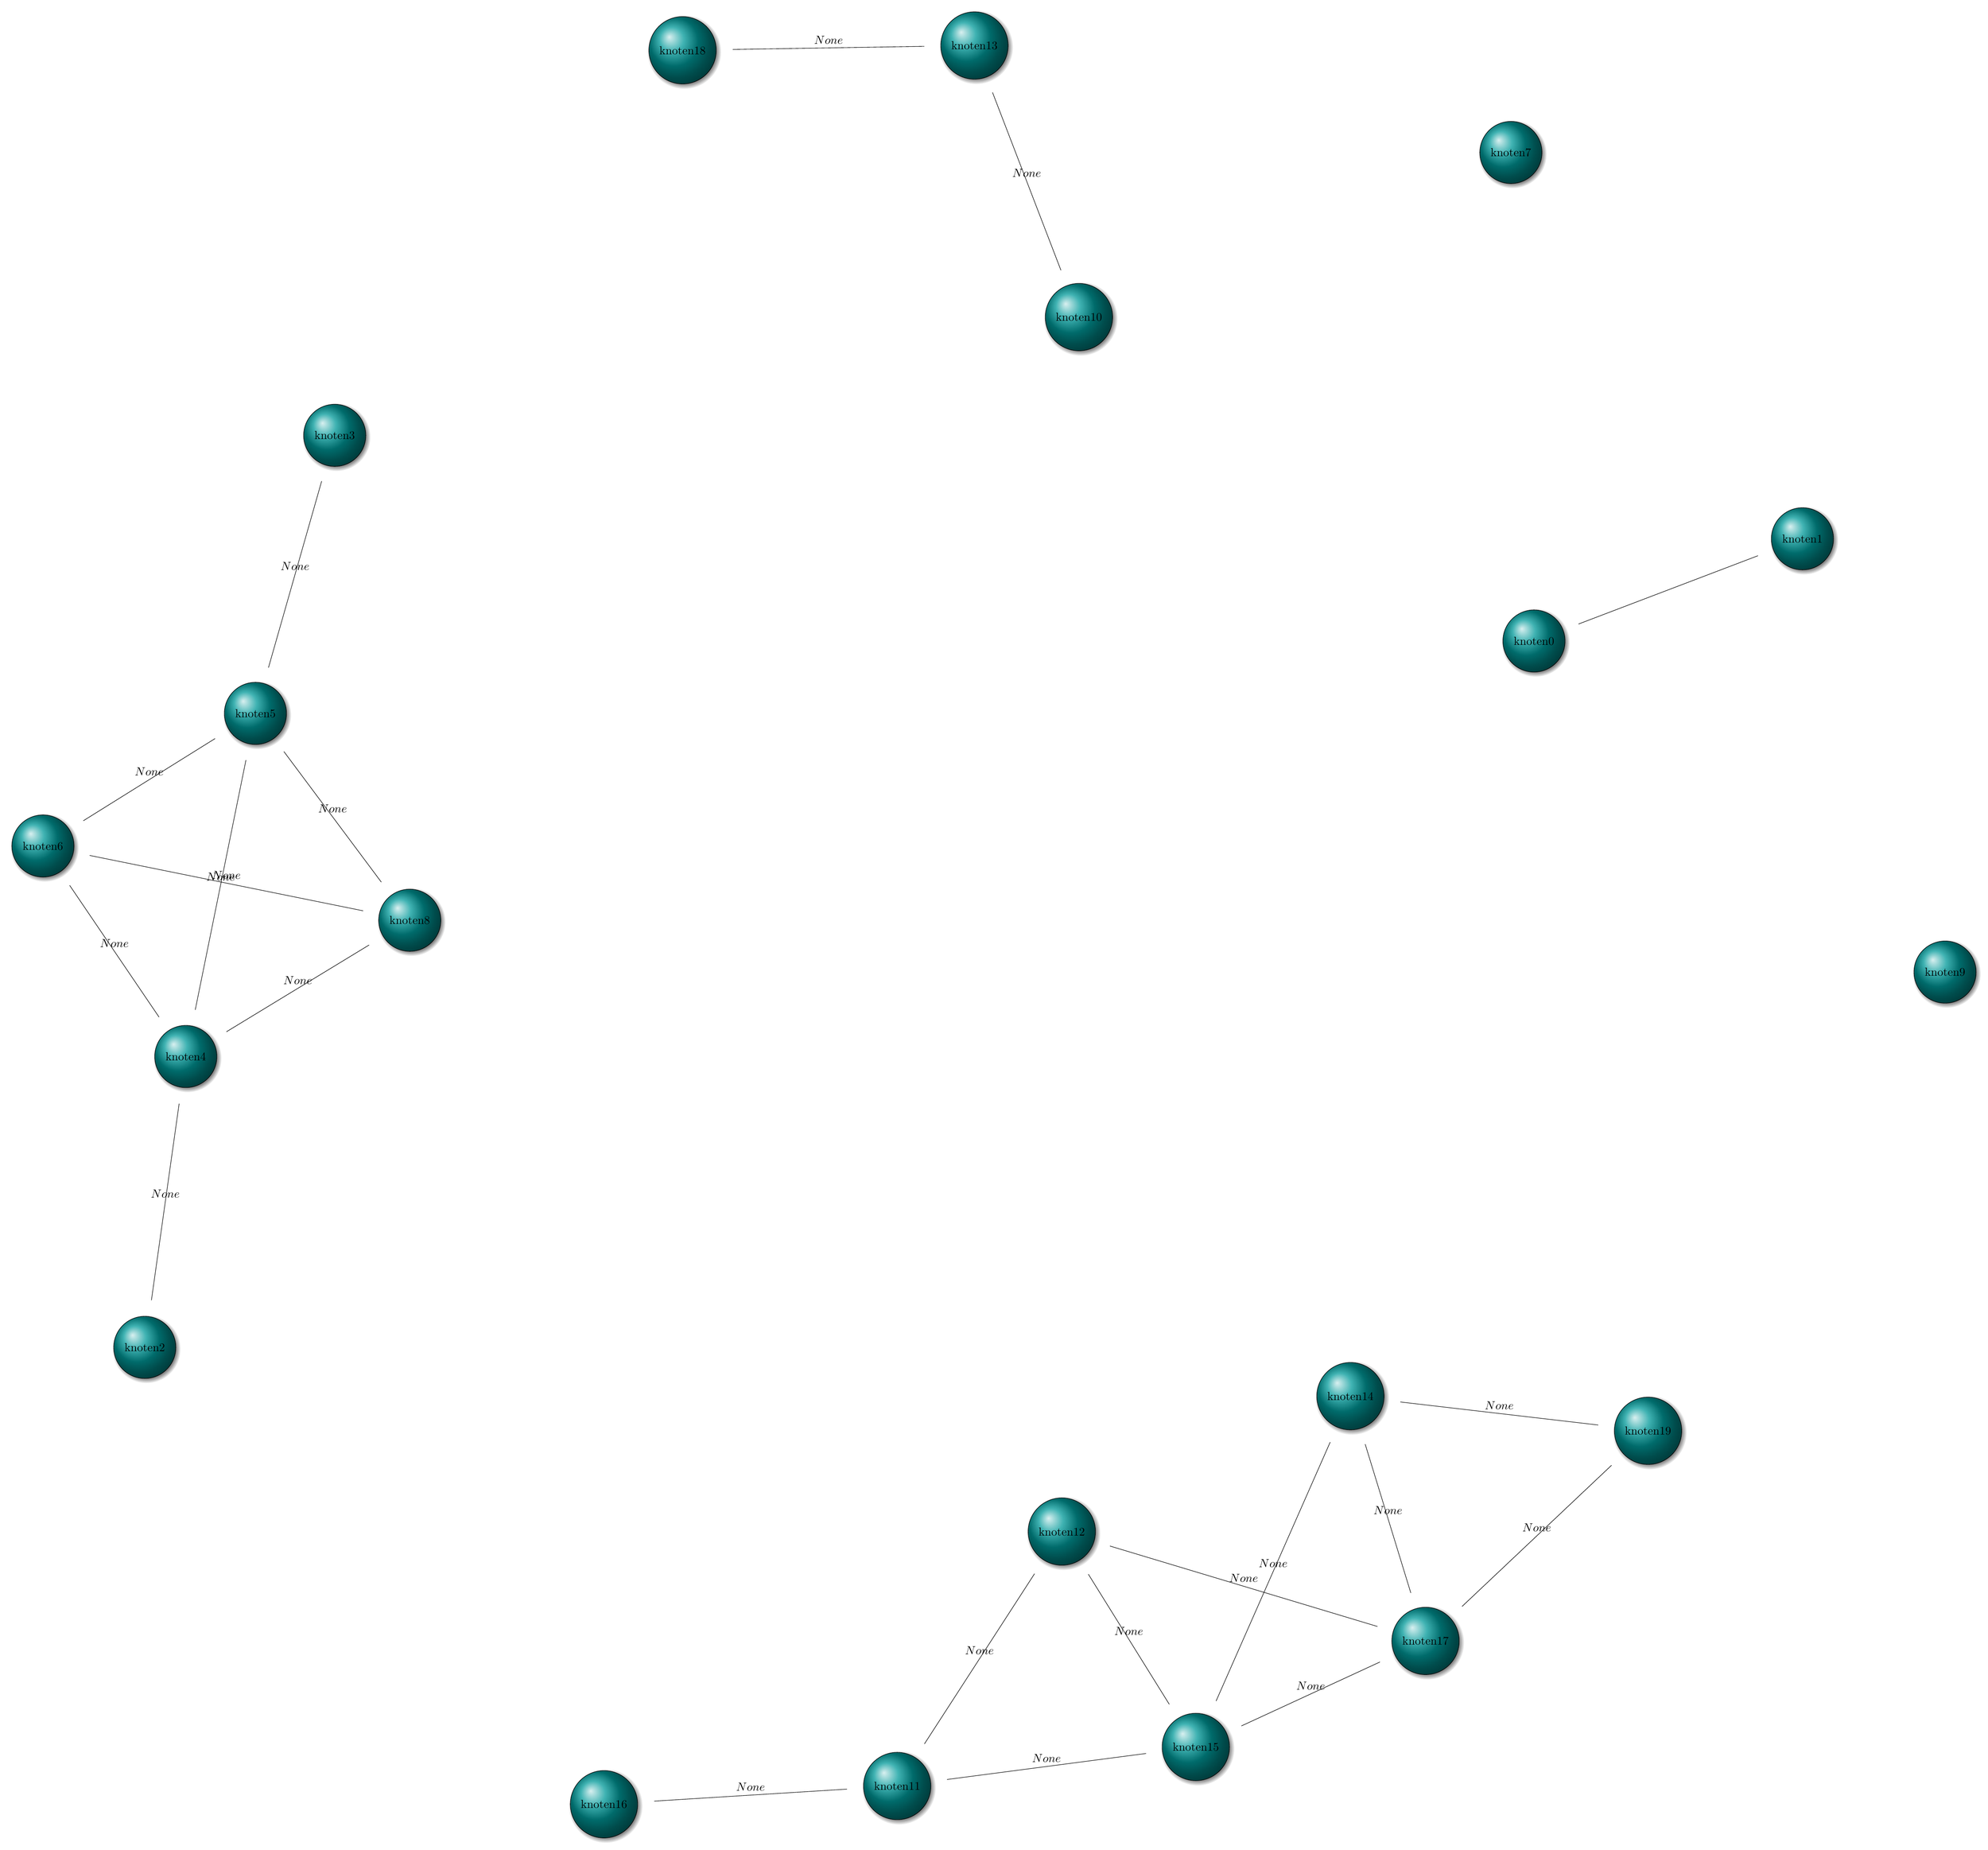
\begin{tikzpicture}[
    knoten/.style={
      shading=ball,
      circle,
      inner sep=.25cm,
      outer sep=.5cm,
      circular drop shadow,
      draw},
    /schriftstueck/.code 2 args={
      \fill[red!50, opacity=#2] #1 rectangle +(.6,.7);
      \foreach \y in {0pt,2pt,4pt,6pt,8pt,10pt,12pt,14pt}
       \draw [yshift=\y, opacity=#2] #1+(0.1,0.1) -- +(0.1,0.1);
      }
    ]


  \node at (49.0460308716, 6.66129183374) (knoten0) [knoten, ball color=cyan!60!black] { knoten0 };
\node at (57.1461513849, 9.74516791669) (knoten1) [knoten, ball color=cyan!60!black] { knoten1 };
\node at (7.13122091437, -14.6508025041) (knoten2) [knoten, ball color=cyan!60!black] { knoten2 };
\node at (12.8621578124, 12.8657989455) (knoten3) [knoten, ball color=cyan!60!black] { knoten3 };
\node at (8.36865196288, -5.87500892425) (knoten4) [knoten, ball color=cyan!60!black] { knoten4 };
\node at (10.4699518268, 4.47700019956) (knoten5) [knoten, ball color=cyan!60!black] { knoten5 };
\node at (4.05874561163, 0.477006740155) (knoten6) [knoten, ball color=cyan!60!black] { knoten6 };
\node at (48.349707264, 21.3998839533) (knoten7) [knoten, ball color=cyan!60!black] { knoten7 };
\node at (15.1265495752, -1.76429890438) (knoten8) [knoten, ball color=cyan!60!black] { knoten8 };
\node at (61.4482870468, -3.3281805361) (knoten9) [knoten, ball color=cyan!60!black] { knoten9 };
\node at (35.317151352, 16.4330958032) (knoten10) [knoten, ball color=cyan!60!black] { knoten10 };
\node at (29.8330394661, -27.8847441985) (knoten11) [knoten, ball color=cyan!60!black] { knoten11 };
\node at (34.8001561215, -20.2076471342) (knoten12) [knoten, ball color=cyan!60!black] { knoten12 };
\node at (32.1644102696, 24.6268238762) (knoten13) [knoten, ball color=cyan!60!black] { knoten13 };
\node at (43.5086587091, -16.1227036378) (knoten14) [knoten, ball color=cyan!60!black] { knoten14 };
\node at (38.8436463259, -26.7070629875) (knoten15) [knoten, ball color=cyan!60!black] { knoten15 };
\node at (20.9866496551, -28.4354213414) (knoten16) [knoten, ball color=cyan!60!black] { knoten16 };
\node at (45.7742843774, -23.5079210861) (knoten17) [knoten, ball color=cyan!60!black] { knoten17 };
\node at (23.3577137858, 24.4839345802) (knoten18) [knoten, ball color=cyan!60!black] { knoten18 };
\node at (52.4878670506, -17.1683074788) (knoten19) [knoten, ball color=cyan!60!black] { knoten19 };





  \path[every node/.style={anchor=south,auto=false}]

        (knoten0) edge  node[] {$$} (knoten1)
(knoten2) edge  node[] {$None$} (knoten4)
(knoten3) edge  node[] {$None$} (knoten5)
(knoten4) edge  node[] {$None$} (knoten5)
(knoten4) edge  node[] {$None$} (knoten6)
(knoten4) edge  node[] {$None$} (knoten8)
(knoten5) edge  node[] {$None$} (knoten6)
(knoten5) edge  node[] {$None$} (knoten8)
(knoten6) edge  node[] {$None$} (knoten8)
(knoten10) edge  node[] {$None$} (knoten13)
(knoten11) edge  node[] {$None$} (knoten12)
(knoten11) edge  node[] {$None$} (knoten15)
(knoten11) edge  node[] {$None$} (knoten16)
(knoten12) edge  node[] {$None$} (knoten15)
(knoten12) edge  node[] {$None$} (knoten17)
(knoten13) edge  node[] {$None$} (knoten18)
(knoten14) edge  node[] {$None$} (knoten15)
(knoten14) edge  node[] {$None$} (knoten17)
(knoten14) edge  node[] {$None$} (knoten19)
(knoten15) edge  node[] {$None$} (knoten17)
(knoten17) edge  node[] {$None$} (knoten19)



   ;



\end{tikzpicture}



\end{document}
